\chapter{Results} \label{ch:results}
\section{Euler Maruyama} \label{sec:dns_v_fp2}

Most SDE’s do not have closed form solutions, but solutions may be computed numerically. The Euler-Maruyama method is a way to create approximate sample paths. 
This method is outlined in \ref{eqn:sde_model_numeric}. A \textit{Python} implementation of this numerical scheme is listed in \ref{appendix:SDEModelSolve}

\begin{figure}[ht]
\begin{subfigure}{.5\textwidth}
  \centering
  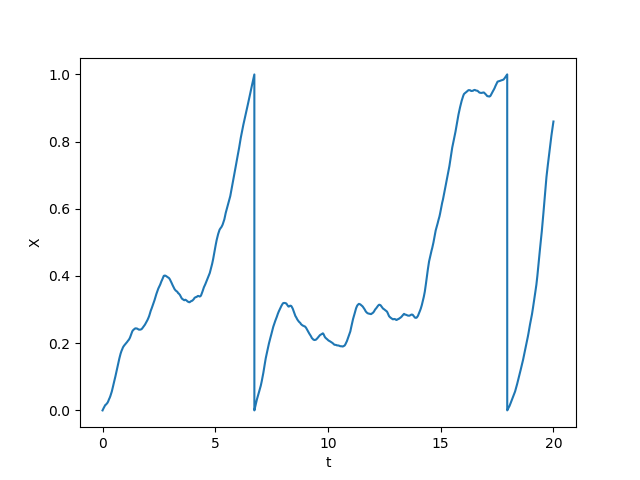
\includegraphics[width=1\textwidth]{/home/ian/Desktop/MSc-Proj/thesistemplate/imgs/x-angle.png}
  \caption{}
\end{subfigure}
\begin{subfigure}{.5\textwidth}
  \centering
  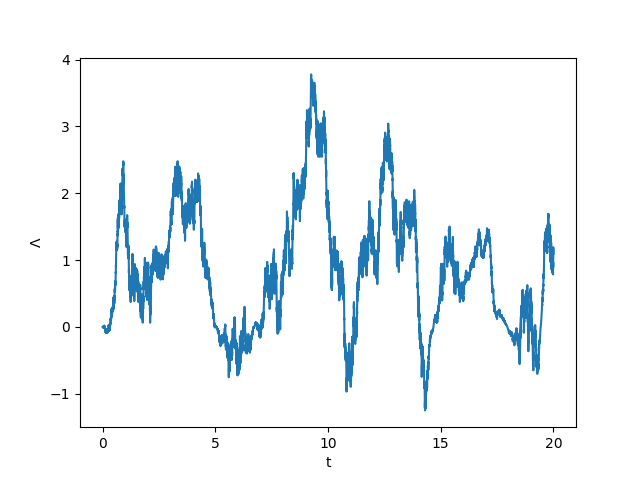
\includegraphics[width=1\textwidth]{/home/ian/Desktop/MSc-Proj/thesistemplate/imgs/lambda.png}
  \caption{}
\end{subfigure}
\caption{(a) Time series of the angle X mod 2$\pi$, (b) Time series of Lyapunov exponent}
\label{fig:sde-em}
\end{figure}

The implemented Euler-Maruyama method with parameters $\omega = 0.5$, $k = 0.5$, $\tau = 0.5$, $D_{Y} = D_{Z} = 2$, $\gamma = 0.5$, $\Delta t = 10^{-6}$, the results of which are shown in Figure \ref{fig:sde-em}
The plot of the normalized X-angle, \ref{fig:sde-em} (a), shows that the X-angle movement to $\pm \pi/2$ as the simulation progresses. The plot of the lyapunov exponent, \ref{fig:sde-em} (b) shows it is positive for
the majority of the simulation, a positive lyapunov exponent indicates chaotic flow.

This method could be used to discover the stationary probability density functions for $\Lambda$ and the angle $X$, by averaging sample paths over many simulations, but this approach converges very slowly. Instead 
the corresponding Fokker-planck equation is more computationally efficient.

\section{Direct Numerical Simulation} \label{sec:dns_v_fp1}

\subsection{DNS vorticity and advection} \label{sec:l_pdf1}
The direct numerical simulation instantaneous vorticity and the advection of the tracer at time $T = 250$ are shown in \ref{fig:omega_theta}, this was based on \textit{matlab} code developed for \cite{main}, and 
listed in \ref{appendix:VorticitySolve}

\begin{figure}[ht]
\begin{subfigure}{.5\textwidth}
  \centering
  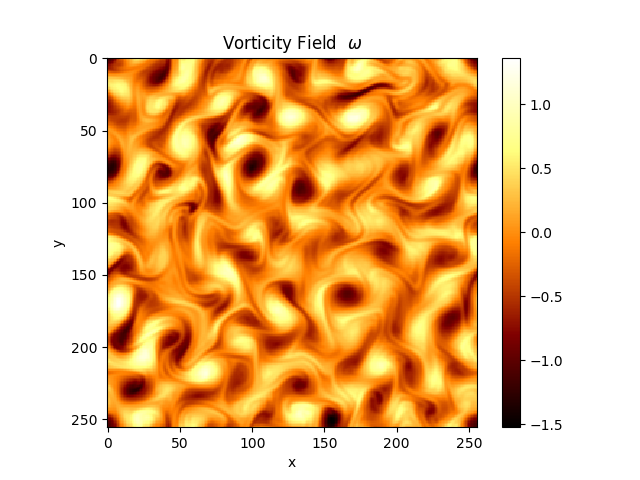
\includegraphics[width=1\textwidth]{/home/ian/Desktop/MSc-Proj/thesistemplate/imgs/vorticity-field-dns.png}
  \caption{}
  \label{fig:sub1_omega_theta}
\end{subfigure}
\begin{subfigure}{.5\textwidth}
  \centering
  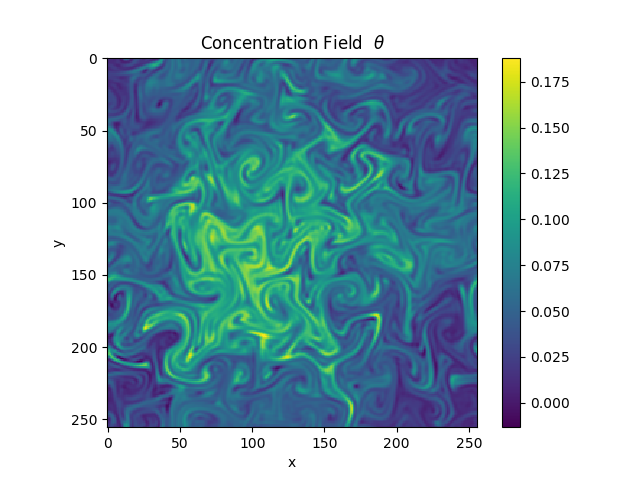
\includegraphics[width=1\textwidth]{/home/ian/Desktop/MSc-Proj/thesistemplate/imgs/concentration-field-dns.png}
  \caption{}
  \label{fig:sub2_omega_theta}
\end{subfigure}
\caption{(a) The vorticity field $\omega$, (b) The concentration field $\theta$}
\label{fig:omega_theta}
\end{figure}



\subsection{DNS statistically steady} \label{sec:l_pdf2}
To extract an accurate distribution for X-angle and the lyapunov exponent $\lambda$ from the DNS, the simulation is run for a long time until it has reached a statistically steady state. 
At each $T_{i} (i \in [1,250])$, $\omega$ and $\theta$ are saved to a file, these are used to create a graphic to visually inspect for the system to have reached a steady state.
Figure \ref{fig:stat-steady} shows the $L^{2}$ norm of the vorticity at each $T_{i}$, 
\begin{figure} 
  \centering
  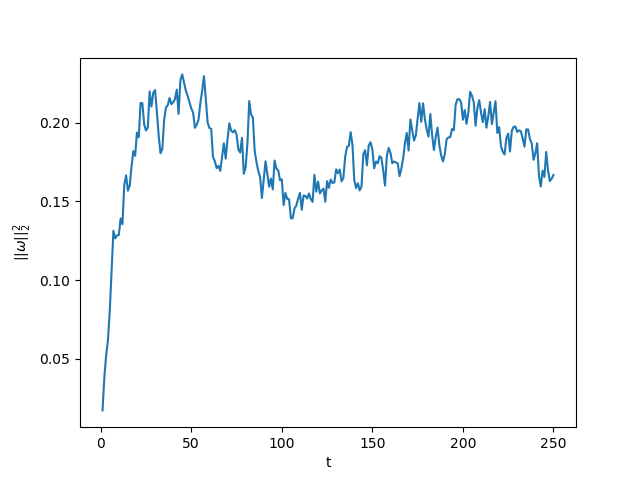
\includegraphics[width=1\textwidth]{/home/ian/Desktop/MSc-Proj/thesistemplate/imgs/stat-steady.png}
  \caption{$L^2$ norm of $\omega$ vs. simulation time}
  \label{fig:sub1_steady}
\label{fig:stat-steady}
\end{figure}

From \ref{fig:stat-steady} we can infer that the flow has reached a statistically homogenous state after $T_{20}$. The data in the files saved from $T_{20}$ to $T_{250}$ are used to 
estimate the PDF of the X-angle and theLyaounov exponent from the DNS.
\subsection{DNS probability density functions, X and $\Lambda$} \label{sec:l_pdf}

The code listed in \ref{appendix:VorticitySolvePostProcessing} estimates the PDF of the X-angle and the Lyaounov exponent from the DNS. Figure \ref{fig:dns-pdfs} shows the estimated PDFs of the 
X-angle and Lyapunov exponent extracted frin the DNS solution to vorticity and advection equation.

\begin{figure}[ht]
\begin{subfigure}{.5\textwidth}
  \centering
  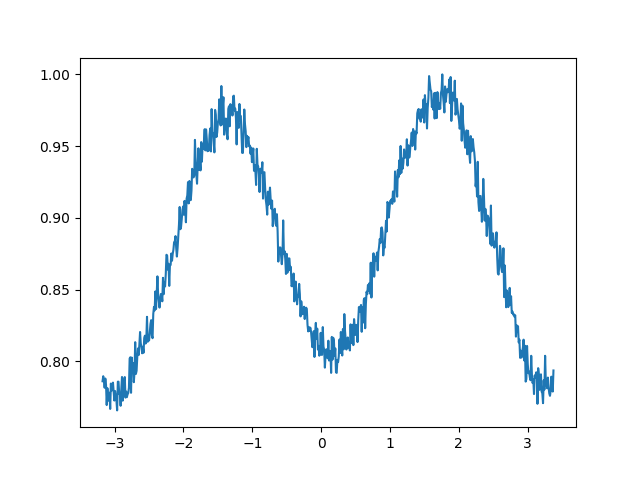
\includegraphics[width=1\textwidth]{/home/ian/Desktop/MSc-Proj/thesistemplate/imgs/angle-x-hist-pdf.png}
  \caption{}
  \label{fig:sub2_dns-pdfs}
\end{subfigure}
\begin{subfigure}{.5\textwidth}
  \centering
  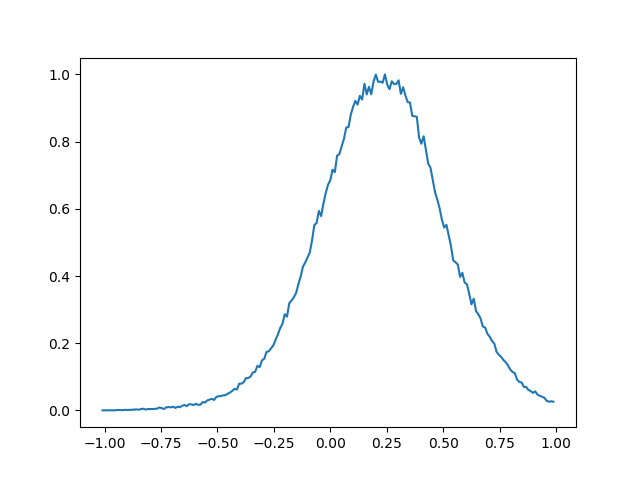
\includegraphics[width=1\textwidth]{/home/ian/Desktop/MSc-Proj/thesistemplate/imgs/lambda-hist-pdf.png}
  \caption{}
  \label{fig:sub1_dns-pdfs}
\end{subfigure}
\caption{(a) The probability density function of the angle $X$, (b)The probability density function of the Lyaounov exponent extracted from the 2-d turbulence simulation}
\label{fig:dns-pdfs}
\end{figure}


\section{Fokker-Planck numerical solution} \label{sec:l_pdf}	
Equation (\ref{eqn:fp}) is solved numerically for the stationary distribution. The marginal distributions of $P_{XY}$ and $P_{YZ}$ are shown in Figure \ref{fig:fp-marginals}.
The distribution of $P_{YZ}$ is Gaussian, which matches up with the numerical implemetation.

\begin{figure}[ht]
\begin{subfigure}{.5\textwidth}
  \centering
  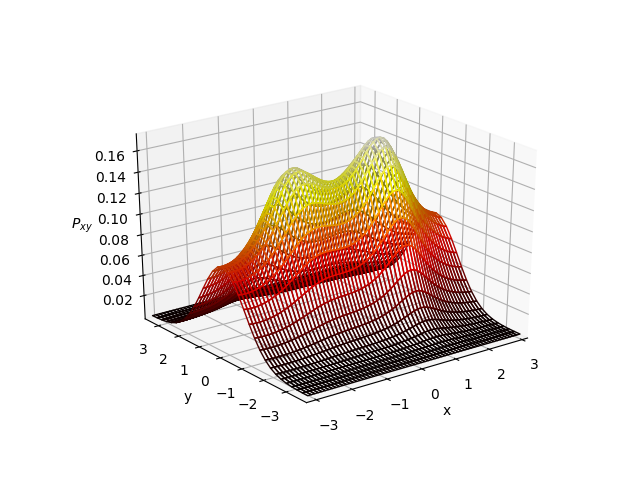
\includegraphics[width=1\textwidth]{/home/ian/Desktop/MSc-Proj/thesistemplate/imgs/fp_p_xy.png}
  \caption{}
  \label{}
\end{subfigure}
\begin{subfigure}{.5\textwidth}
  \centering
  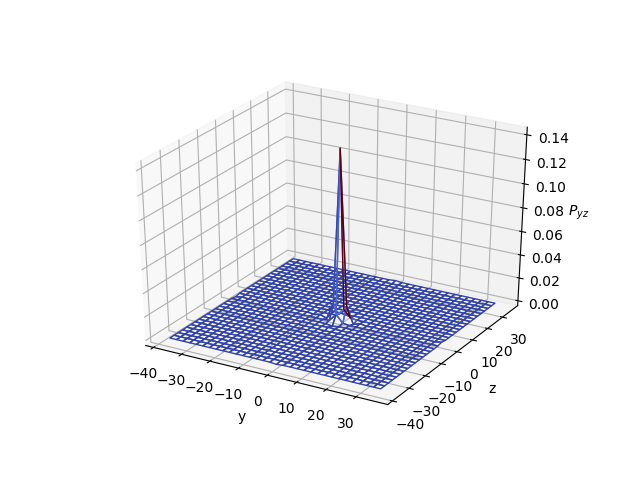
\includegraphics[width=1\textwidth]{/home/ian/Desktop/MSc-Proj/thesistemplate/imgs/fp_p_yz.png}
  \caption{}
  \label{}
\end{subfigure}
\caption{The marginal probability distribution got from the stationary solution to the Fokker-Planck equation, (a) joint marginal $x-y$, (b) joint marginal $Y-Z$}
\label{fig:fp-marginals}
\end{figure}

The more import result is the marginal distribution of $X$ , define in Equation (\ref{eqn:x-marginal}) and the marginal distribution of $\Lambda$ defined in Equation (\ref{eqn:lambda-marginal}), shown in Figure (\ref{fig:fp-single-marginals})

\begin{figure}[ht]
\begin{subfigure}{.5\textwidth}
  \centering
  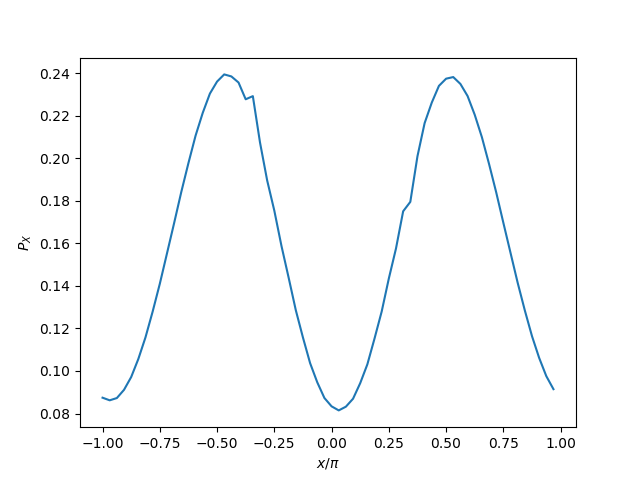
\includegraphics[width=1\textwidth]{/home/ian/Desktop/MSc-Proj/thesistemplate/imgs/fp_p_x.png}
  \caption{}
  \label{}
\end{subfigure}
\begin{subfigure}{.5\textwidth}
  \centering
  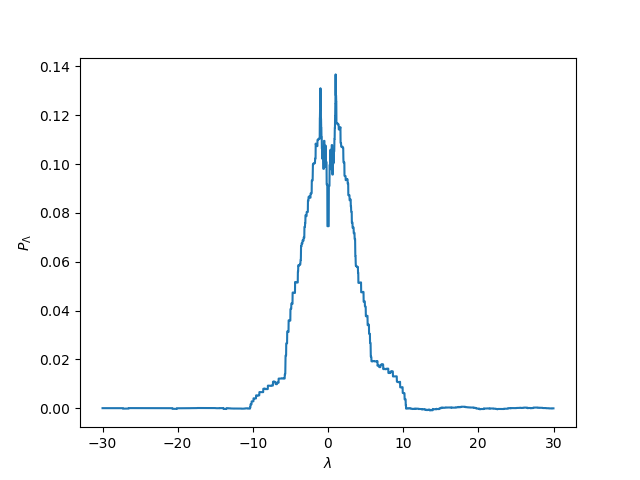
\includegraphics[width=1\textwidth]{/home/ian/Desktop/MSc-Proj/thesistemplate/imgs/fp_p_lambda.png}
  \caption{}
  \label{}
\end{subfigure}
\caption{The distribution of the X-angles from Fokker-Planck (a) and The distribution of the Lyaounov exponents from Fokker-Planck (b)}
\label{fig:fp-single-marginals}
\end{figure}

The distribution of the $X$ angles are whien in Figure. \ref{fig:fp-single-marginals}(a). This has two maxima close to $X = \pm \pi/2$. They do not line up exactly at $\pm \pi/2$ due to the correlcation $k = 0.5$ between the random terms and the drift $\omega = 0.5$.
Setting $ k = \omega = 0$ the distribution of the $X$ angle aligns with $\pm \pi/2$. From this result we can conclude most probable alignment of the $X$-angle is close to $\pi/2$. 
This reveals the most likely direction the vector $\mathbf{X}_{(+)}$ (the positive eigenvector of the rate-of-strain matrix $\mathcal{S}$) will point.

Figure. \ref{fig:fp-single-marginals}(b) shows the distribution of the Lyapunov exponent. THis distribution is slightly asymmetric to the right with the first moment of the distribution positive. 

From these results we can conclude the most likely direction of the stretching direction is close to $\pi/2$ with a positive Lyaounov exponent.
